% Copyright (C)  2015  Alexander Jankowski, Philipp Hacker.
% Permission is granted to copy, distribute and/or modify this document
% under the terms of the GNU Free Documentation License, Version 1.3
% or any later version published by the Free Software Foundation;
% with no Invariant Sections, no Front-Cover Texts, and no Back-Cover Texts.
% The lincense itself can be found at <https://www.gnu.org/licenses/fdl-1.3>.

\documentclass[numbers=noenddot,a4paper,notitlepage,twoside,BCOR15mm]{scrartcl}
%\documentclass[numbers=noenddot,12pt,a4paper]{scrartcl}

\usepackage{ifoddpage}
\usepackage[infoshow]{tabularx}
\usepackage{fancyhdr}
\usepackage[greek,ngerman]{babel}
\usepackage[T1]{fontenc}
\usepackage[utf8]{inputenc}
\usepackage{libertine}
\usepackage{ziffer}
\usepackage{graphicx}
\usepackage{units}
\usepackage[infoshow]{tabularx}
\usepackage[all]{xy}
\usepackage{amsmath}
\usepackage{amssymb}
\usepackage{wrapfig}
\usepackage{upgreek}
\usepackage{esint}
\usepackage{float}
\usepackage[font=small,labelfont=bf]{caption}
\usepackage{subcaption}
\usepackage{lscape}
\usepackage[backref=page]{hyperref}
\usepackage{cleveref}
\usepackage{csquotes}

\renewcommand{\headrulewidth}{0.1pt}
\renewcommand{\footrulewidth}{0.1pt}
\newcommand{\name}{\text{Philipp Hacker}} %TODO Name des Protokollanten eintragen

\renewcaptionname{ngerman}{\figurename}{Abb. }
\renewcaptionname{ngerman}{\tablename}{Tab.}

\setlength{\parindent}{0pt}

\newcommand{\nummat}[1]{\left[\text{#1}\right]}
\newcommand{\num}[1]{$\left[\text{#1}\right]$}
\newcommand{\degree}{^\circ}
\newcommand{\diff}{\textnormal{d}}
\newcommand{\tenpo}[1]{ 10^{#1}}
\newcommand{\greek}[1]{\greektext#1\latintext}
\newcommand{\ix}[1]{_\text{#1}}
\newcommand{\imag}{\mathbf{i}}
\newcommand{\tilt}[1]{\textit{#1}}
\newcommand{\grad}[1]{\textit{grad}\left(#1\right)}
\newcommand{\divergenz}[1]{\textit{div}\left(#1\right)}
\newcommand{\euler}{\mathnormal{e}}
\newcommand{\fett}[1]{\textbf{#1}}
\newcommand{\einnup}{\hspace{0.2cm}}
\newcommand{\einnum}{\hspace{-0.2cm}}
\newcommand{\zentriert}[1]{\begin{center}#1\end{center}}

\title{Protokoll: Reflektron/\\\tilt{time of flight}-Massespektrometrie} %TODO Name des Versuchs eintragen
\author{Alexander Jankowski, Philipp Hacker}
\date{\today}
\pagestyle{fancy}
\fancyhead[C]{\thepage}
\fancyhead[R]{\name}
\fancyfoot[C]{\thepage}
\fancyhead[L]{Abschnitt \thesection}

\begin{document}
	\maketitle
	\begin{center}
		Betreuer: Marco Rosenbusch \\ %TODO Name des Betreuers eintragen
		Versuchsdatum: 4.11.2015 \\ %TODO Datum des Versuchs eintragen
		\begin{table}[h]
			\centering
			Note: %TODO Gute Note erhalten :)
			\begin{tabularx}{1.5cm}{|X|}
				\hline \\ \\
				\hline
			\end{tabularx}
		\end{table}
	\end{center}
	\vspace*{\fill}
	\tableofcontents
	\vfill
	\clearpage
	\section{Motivation}

		Die Messungen von Präzisionsmassenspektrometer sind ein wichtiger Bestandteil der Zusammenarbeit von Theorie und Praxis. Insbesondere gilt dies für astrophysikalische Zusammenhänge (siehe: Experiment \tilt{ISOLTRAP} am Kernforschungszentrum \tilt{CERN}). Die Genauigkeit mit welcher Massen heute bestimmt werden - und das geschieht auf die verschiedensten Weisen mit den unterschiedlichen Hintergründen - macht es möglich, Voraussagen aus bspw. der Kernphysik experimentell nachzuvollziehen und Vorausblicke in die zukünftige Entdeckung von Isotopen/Isobaren \dots zu tätigen.

	\clearpage
	\section{Physikalische Grundlagen}

		Die in diesem Versuch benutzte Methode der Auflösung und Messung von Massen oder Masse-zu-Ladungs-Verhältnissen ist die der Massenspektrometrie, insbesondere der \tilt{time of flight-Massenspektromertie}.\\
		Dabei werden die zu betrachtenden Teilchen - sein es nun Cluster von mehreren Dutzend Atomen, Moleküle oder deren Monomere bzw. Ionen - in Richtung eines Detektors/Analysators über ein elektrisches Feld beschleunigt. Dabei ist der Strom von, beispielsweise Ionen, möglichst auf eine Bahn fokussiert und quantisiert, sodass hinter der feldfreien Strecke des \tilt{Analysators} die, durch den restlichen Aufbau transmittierten Teilchen nach ihrer Flugzeit im Detektor aufgelöst werden. Die zeitliche Trennung von, notwendigerweise geladenen Probesubstanzen ist Folge der unterschiedlichen Beschleunigungen und damit Geschwindigkeiten aufgrund verschiedener Massen-zu-Landungs-Verhältnissen.\\
		Die Beschleunigung über ein Kondensator-Feld aus \autoref{eq:feld} ergibt die kinetische Energie in \autoref{eq:kinet}. Daraus erkennt man bereits: Teilchen mit gleichen Ladungen aber unterschiedlichen Massen werden verschieden stark beschleunigt, da die kinetische Energie in Abhängigkeit der Potentialdifferenz konstant ist. Vereinfacht man das Problem eines einstufigen \tilt{tof-MS} in einer Dimension - dh. nimmt man an, es gäbe nur eine Stufe $d\ix{1}$ für die Beschleunigung, der Analysator hätte die Länge $d$ und die Ionen würden mit dem Ortsunterschied $\Delta x$ in elektrische Feld mit der thermischen Anfangsgeschwindigkeit aus $qU\ix{th,x}$ eintreten - so ergibt sich die Gesamtflugzeit $t\ix{tof}$ aus der Analysator-Laufzeit $t\ix{d}$ und der Beschleunigungsdauer $t\ix{1}$ in \autoref{eq:tof}.

			\begin{align}
				E\ix{e}=&\frac{U}{d} \label{eq:feld}\\
				E\ix{kin}=qU&=\frac{mv^2}{2} \label{eq:kinet}\\
				\sqrt{\frac{m}{w}}\propto t\ix{tof}=t\ix{1}+t\ix{d}=\sqrt{\frac{m}{q}}\frac{1}{E}&\left[\sqrt{2v\ix{2}}\pm\sqrt{U\ix{th,x}}\right]+\frac{d}{2\sqrt{v\ix{2}}} \label{eq:tof}\\
				v\ix{2}=U\ix{th,x}+&E\left(\frac{d\ix{1}}{2}-\Delta x\right)
			\end{align}

		Das Prinzip der \tilt{tof-MS} greift darauf zurück, das unterschiedlich schnelle Teilchen für eine feldfreie Strecke verschiedene Flugzeiten $t\ix{1}(m\ix{1},q\ix{1}),t\ix{2}(m\ix{2},q\ix{2}),\dots$ benötigen. Das Beispiel in \autoref{eq:tof} kann auf verschiedene Weisen erweitert und verbessert werden. Um den Ortsfokus zu verbessern, dh. den Einfluss von $\Delta x$ und Ablenkungen von der Aufbau-Achse zu minimieren, benutzt man mehrstufige \tilt{tof-MS} und Ionen-Optiken, welche den Teilchenstrom kanalisieren. Wegen der Ortsunschärfe von gleichen Teilchen in der Quelle liegen auch jeweils unterschiedliche Beschleunigungsstrecken vor, weswegen eine 'Verschmierung' der Flugzeit von einzelnen Spezies in Kombination mit der thermischen Verteilung auftritt. Damit dieser Zeitfokus gegeben ist (gleiche Ionen sind zu einer bestimmten Zeit am gleichen Ort), baut man mehrstufige \tilt{tof-MS} mit kleinen und sehr großen Potentialgradienten. Die Auswirkungen von $E\ix{kin,th}$ und $\Delta x$ verschwinden (min. näherungsweise bis zur 2. Ordnung), wobei sich die Gesamtflugdauer um eine Zeit auf der zweiten \dots n-ten Beschleunigungsstrecke erhöht. Insbesondere ist dies der Fall für $d=d\ix{1}$  in der \autoref{eq:tof}.

			\begin{figure}[t]
				\centering
				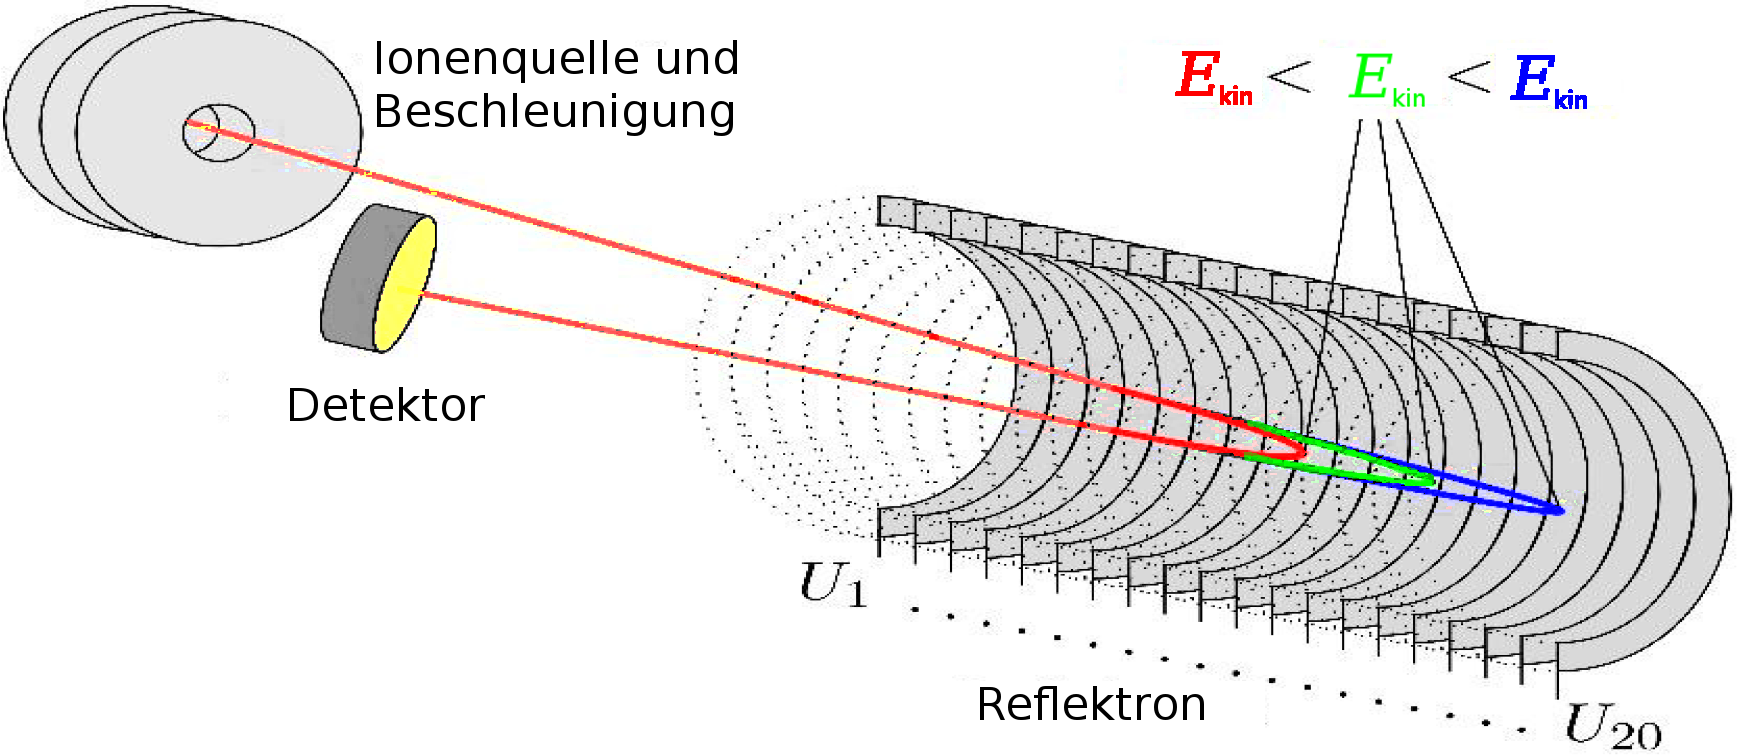
\includegraphics[width=0.8\textwidth]{einspiegel.png}
				\caption{Ein-Spiegel Reflektron mit Ionenquelle, Beschleunigungssektoren und einem Detektor. Hier ist die Abhängigkeit des Eindringens von der kinetischen Energie gezeigt. \cite{EMAUGreifswaldReflektron}}
				\label{img:reflektron1}
			\end{figure}

		Beim sogenannten \tilt{Reflektron} handelt es sich um eine elektrostatische Ionenfalle bzw. Flasche - angelehnt an die elektromagnetische Beschreibung von Elektronen-Bewegungen in Plasmen unter Einfluss eines inhomogenen, gekrümmten Magnetfeldes - welche ein inhomogenes Feld durch viele unterschiedliche Elektroden hintereinander erzeugt. Dieser koaxiale Spiegel reflektiert einfallende Ladungsträger entweder in Richtung des Detektors oder auf einen zweiten, ihm gegenüberliegenden Spiegel (Abhängigkeit von Form des Feldes und der Einfallsrichtung). Teilchen der gleichen Massen-zu-Ladung-Spezies aber mit unterschiedlichen Geschwindigkeiten dringen verschieden weit in das Spiegel-Feld ein. Im speziellen werden sie im Bremsbereich verlangsamt und dann in einem Abschnitt eines flacheren Feldgradienten 'korrigiert' und reflektiert. Dabei dringen zum Beispiel schnellere Teilchen der selben Masse und Ladung tiefer in den Reflektron ein und legen damit mehr Weg zurück, als ihre langsameren Partner. Über die Reflektion werden sie jedoch wiederum stärker und länger beschleunigt, was ihnen ihre Einfallsgeschwindigkeit verleiht. Insgesamt ist bzw. sollte das Reflektron-Feld so geformt sein, dass eben diese, im Impulsraum 'verschmierte' Population einer Probesubstanz an einem fixen Ort innerhalb eines Aufbaus mit 2 Spiegeln zusammenkommt. Unter Umständen ist in Aufbauten mit einem Spiegel ist dieser Ort die Detektoroberfläche.

			\begin{figure}[b]
				\centering
				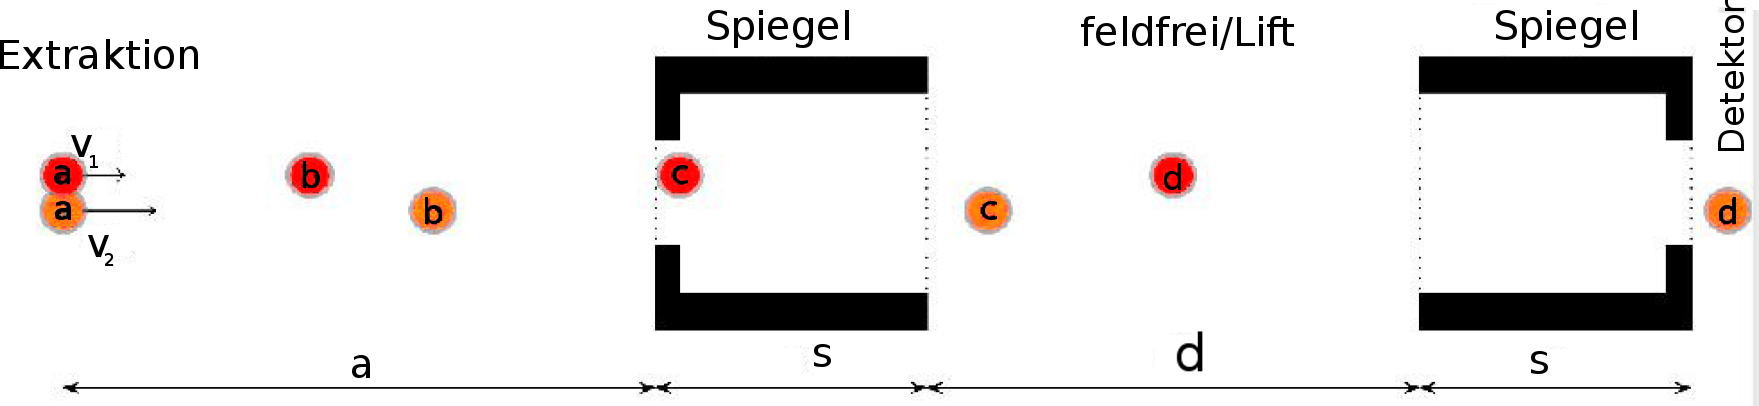
\includegraphics[width=\textwidth]{zweispiegel.png}
				\caption{Zwei-Spiegel Reflektron mit internen Abmessungen. Eingezeichnet ist die Ionenbewegung mit 2 unterschiedlichen Geschwindigkeiten $v\ix{2}>v\ix{1}$ durch den Aufbau. Das schnellere Teilchen tritt dabei ohne Reflektion aus (siehe \autoref{eq:speicher}). \cite{EMAUGreifswaldReflektron}}
				\label{img:reflektron2}
			\end{figure}

		Die \autoref{img:reflektron1} und \autoref{img:reflektron2} zeigen den schematischen Verlauf von Ionen aus der Quelle/einer Ionenfalle, in welcher sie gespeichert und selektiert wurden, in einen Ein-Spiegel/Zwei-Spiegel-Reflektron bis auf den Detektor. Zwischen beiden Spiegeln befindet sich eine feldfreie Driftstrecke bzw. ein elektrostatischer 'Lift', welcher den einfallenden/reflektierten Ionen ein neues Bezugspotential verleiht und somit das Eindringen oder Verlassen des Reflektrons ermöglicht. Das Verhältnis von kinetischen Energien, Massen und damit Geschwindigkeiten zweier Ionenspezies, welche im Reflektron verbleiben sollen, ergibt sich mit den Größen $a$, $s$ und $d$ welche \autoref{img:reflektron2} entnommen werden können, in \autoref{eq:speicher}.


		\begin{align}
			\frac{v\ix{1}}{v\ix{2}}=\sqrt{\frac{E\ix{kin,1}m\ix{2}}{E\ix{kin,2}m\ix{1}}}<\frac{a+s+d}{a+s} \label{eq:speicher}
		\end{align}

		Bei einem Multireflexions-Massenspektrometer nutzt man die vielfache Durchquerung des feldfreien Driftbereichs um dicht beeinander liegende Geschwindigkeiten und damit kinetischen Energien deutlich aufzutrennen. Dies spielt eine wichtige Rolle für das Auflösungsvermögen des Experiments, welches als

			\begin{align}
				R=\frac{m}{\Delta m} \label{eq:aufloes}
			\end{align}

		definiert wird. Dabei ist $\Delta m$ unterschiedlich interpretierbar: nach der FWHM-Methode (\tilt{full width at half maximum}) entspricht dieser Wert der Halbwertsbreite des \tilt{gauß'schen} Normalverteilungs-Peaks um die Wahre Masse im Spektrum. Über die 10\% bzw. 50\%-Methode definiert man die kleinstmögliche, unterscheidbare Massendifferenz $\Delta m$ als den Abstand zweier \tilt{Gauß}-Peaks die sich bei einem Zehntel bzw. der Hälfte ihrer Höhe schneiden.\\
		Insbesondere wird $R$ für einen Reflektron-Versuch, mit der Reflexions-Zeit $t\ix{n}$, der Zeit von Quelle zur Falle $t\ix{s}$, sowie $\Delta t\ix{s}$ und $\Delta T$ den Fehlern der Flugzeiten bei $n$-facher Reflexion zu

			\begin{align}
				R=\frac{t\ix{s}+t\ix{n}}{2\sqrt{\Delta t\ix{s}^2+n^2\Delta T}}\,\, . \label{eq:fehler}
			\end{align}

		Um ein \tilt{tof-MS} zu kalibrieren, misst man in dem Aufbau das Spektrum zweier sehr genau bekannter Massen $m\ix{1}$,$m\ix{2}$. Der Zusammenhang zwischen den gemessenen Flugzeiten$t\ix{1}$,$t\ix{2}$, den systematischen Fehlern (zusammengefasst) $t\ix{0}$ und den skalierenden Faktoren $\sigma\ix{tof}$ ergibt sich in \autoref{eq:zeit}. Eine Messung einer unbekannten Masse setzt damit aus den aufgelösten Größen der Fehler und dem erhaltenen Spektrum zusammen, was in \autoref{eq:abszeit} angeführt ist.

			\begin{align}
				t\ix{1}=\sigma\ix{tof}&\sqrt{m\ix{1}}+t\ix{0}\,\,, \,\,\,\, t\ix{2}=\sigma\ix{tof}\sqrt{m\ix{2}}+t\ix{0} \label{eq:zeit}\\
				\sigma\ix{tof}=\frac{t\ix{1}-t\ix{2}}{\sqrt{m\ix{1}-\sqrt{m\ix{2}}}}\,\,& , \,\,\,\, t\ix{0}=\frac{1}{2}\left(t\ix{1}+t\ix{2}-\frac{\sqrt{m\ix{1}}+\sqrt{m\ix{1}}}{\sqrt{m\ix{1}}-\sqrt{m\ix{1}}}\left(t\ix{1}-t\ix{2}\right)\right) \nonumber \\
				&\sqrt{m}=\frac{t-t\ix{0}}{\sigma\ix{tof}} \label{eq:abszeit}
			\end{align}

	\clearpage
	\section{Durchführung}

		Der Aufbau dieses Versuches ist in \autoref{img:aufbau} gezeigt. Nach der Erzeugung in der Quelle treten die geladenen Teilchen in ein Kondensator-Feld zur Beschleunigung in Richtung einer Ionenfalle ein. Dabei ist eine sogenannte \tilt{Paulfalle} verwendet worden, um die zu untersuchenden Ionen aus der Quelle zu speichern und zu selektieren. Dies geschieht mittels des Schemas aus \autoref{img:paulfalle}, wobei sich die Potentiale auf der Hauptkammer und den Endkappen aus dem Gleichspannungsanteil $U$ und der Wechselspannung $\tilde{V}$ zusammen setzen. Diese sind so kalibriert, das sie nur einen kleinen Bereich aus dem Spektrum von $\sqrt{m/q}$ im Inneren halten, der Rest driftet auf die Elektroden. Die Paulfalle ermöglicht es also, gespeicherte Teilchen - sofern die Lebensdauer ausreicht - auf gewünschte Arten zu manipuliere, e.g. Ionisieren.

		\begin{figure}[h]
			\centering
			\begin{subfigure}{0.35\textwidth}
				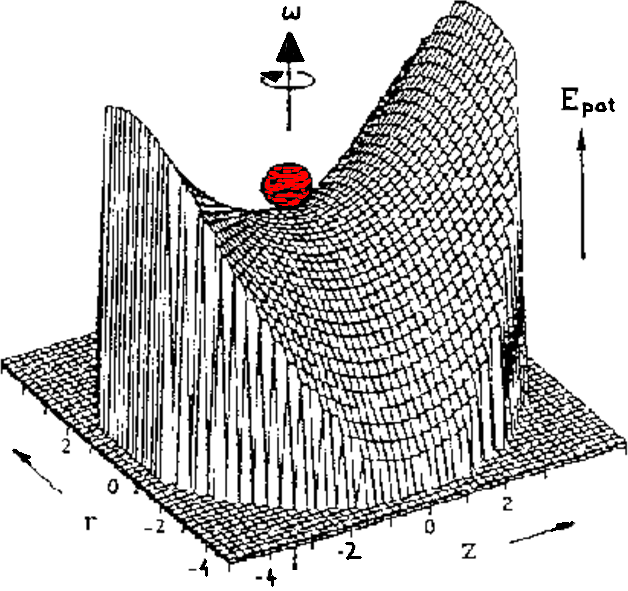
\includegraphics[width=\textwidth]{paulpotential.png}
				\caption{}
				\label{img:potential}
			\end{subfigure}
			\begin{subfigure}{0.4\textwidth}
				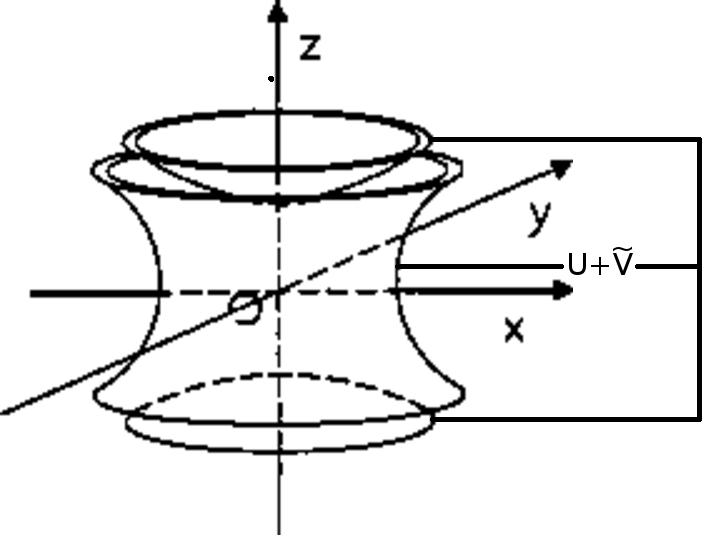
\includegraphics[width=\textwidth]{paulfalle.png}
				\caption{}
				\label{img:paulfalle}
			\end{subfigure}
			\caption{\fett{(a):} Potential der Paulfalle mit gyrierendem Teilchen. \fett{(b):} Allgemeiner Aufbau einer Paulfalle mit Endkappen und Potentialen $U$,$\tilde{V}$ \cite{UMainzReflektron}}
		\end{figure}

		\begin{figure}[t]
			\centering
			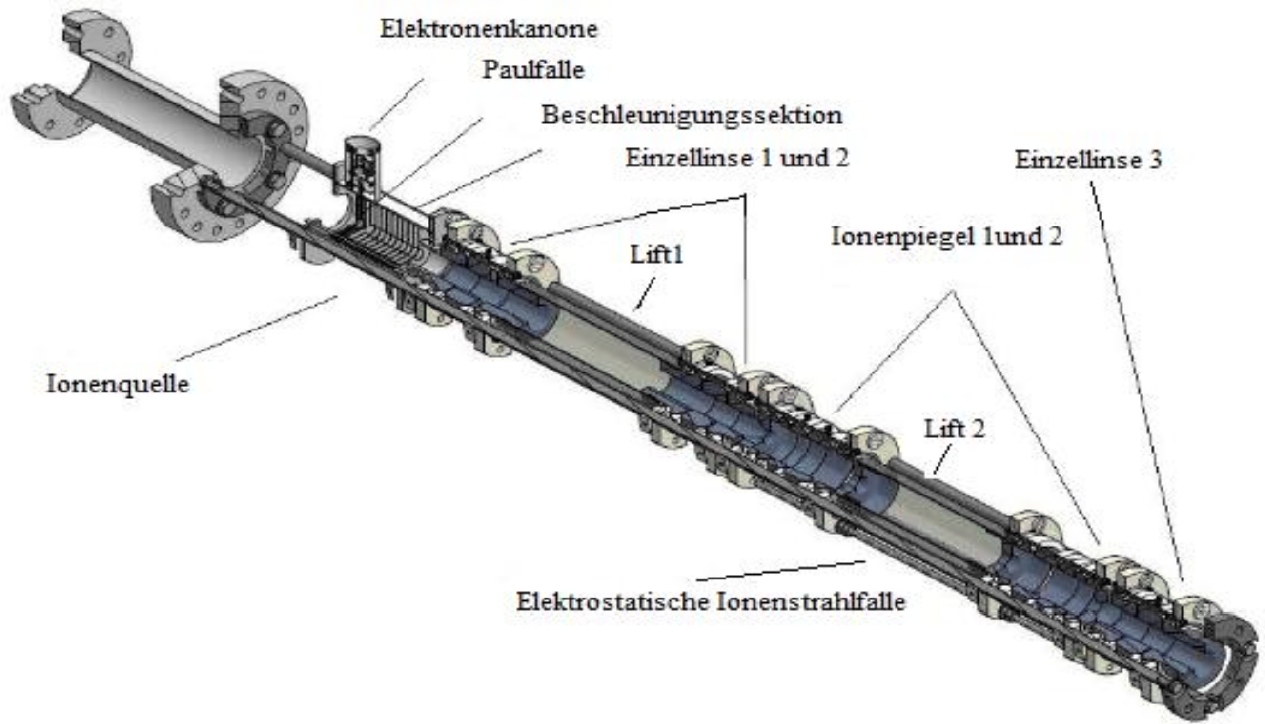
\includegraphics[width=\textwidth]{aufbau.png}
			\caption{Gyration eines Ions innerhalb des Paulfallen-Potentials. \cite{UMainzReflektron}}
			\label{img:aufbau}
		\end{figure}

		Nach der Speicherung gelangt die Probesubstanz in die bereits besprochene mehrstufige Beschleunigungssektion. Dort erhalten die Teilchen ihre kinetische Energie in Abhängigkeit von der Masse und Ladung. Dieser Bereich ist ebenso mit komplizierten Wechselfelder (explizit gegenläufig, um den Strahl um die optische Achse zu 'halten') beschaltet, da die Ionen ansonsten auf die Wände der Kammer treffen würde und kein Signal auf dem Detektor erzeugen könnten. Ionen-optische Linsen fokussieren den austretenden Teilchenstrahl auf den Eintrittsort des \tilt{Lifts}: dieser schaltet vom Potential der Beschleunigungssektion auf ein günstigeres, für den weiteren Aufbau geeigneteres Potential (i.A. niedriger, da bis hierher Spannung von mehreren Hundert Volt bis hin zu Kilo-Volt angelegt wurden) sobald die Ionen in diesen eintreten. Somit erhalten die Teilchen ein neues Bezugspotential, ohne dabei Konsequenzen für ihre Geschwindigkeit zu erfahren.\\
		Anschließend tritt die Probesubstanz in den eigentlichen Reflektron ein. Zum Eingang ist dessen interner Lift - und auch später die eigentliche Driftstrecke - und der vordere Spiegel abgeschaltet bzw. auf Bezugspotential. Danach wird wie zuvor verfahren: die Ionen werden nach Eintritt über den Lift 'angehoben', damit sie in der elektrostatischen Flasche nicht austreten können. Das heißt explizit, dass deren Bezugspotential kleiner als die Reflexionsspannung ist. Nach einer endlichen Zeit können die reflektierenden Teilchen durch das erneute 'hochschalten' des Lifts austreten und auf einen Detektor treten.\\
		Während der Durchführung des Versuchs wurde sich mit den unterschiedlichen Bauteilen und Steuerfunktionen vertraut gemacht. Dafür wurden die verschiedenen Zeiten zum Speichern, Lift-Anheben und Reflexionen variiert. Insbesondere war es die Aufgabe, Flugzeit und damit Masse des Stickstoff-Ions zu bestimmen. Dafür verwendet werden die geeichten Massen (als exakt angenommenen) anderer Ionensorten aus der Luft. Die Aufgabe dafür war , die Reflexionszeit der Probesubstanz bis auf eine Genauigkeit von 100 Umläufen, dh. das hundertfache der einfachen Durchlaufzeit, zu bestimmen. Im Spektrum erhält man dadurch einen sehr deutlichen und weit von anderen Massen getrennten Peak für das gesuchte Ion. Die Resultate (dreimalige Aufnahme) der anderen Teilchen werden zur Eichung genutzt (siehe \autoref{eq:abszeit}).

	\clearpage
	\section{Auswertung}

	\subsection{Bestimmung der Umlaufzeiten der Ionensorten}
	
	Um die verbesserte Massenauflösung des Multireflektrons nutzen zu können, muss zuerst die Umlaufzeit $t_\mathrm{U}$ der einzelnen Ionensorten bestimmt werden. Die Umlaufzeit gibt an wie lange das Ion braucht um eine volle Periode im Multireflektron zu vollführen. Hierfür wird die Schaltdauer des Liftes zwischen den Ionenspiegeln solange variiert, bis das Ionensignal wieder auf dem Detektor gemessen wird. Es wird ein Signalpeak betrachtet und seine Position notiert. Für die nächste Messung wird die Liftzeit Schrittweise um das $n$-fache erhöht, so dass die Ionen im Reflektron weitere Perioden vollführen. Wurde die Zeit richtig gewählt, so verschiebt sich der Peak im Flugzeitspektrum bei mehreren Perioden nicht. Ist dies doch der Fall wird die Liftzeit angepasst, bis das Signal bei $100$ Umläufen noch an der selben Stelle im Flugzeitspektrum ist. Dies wird für die Ionen N$_2^+$, O$_2^+$ und N$^2$H$^+$ durchgeführt. Die Umlaufzeiten sind in Tab.\ref{tab:umlauf} dargestellt. Die Abb.\ref{abb:N2}-\ref{abb:N2H} zeigen ein Spektrum der jeweiligen Ionensorte.
	
	\begin{table}[h]
		\centering
		\caption{Die gemessenen Umlaufzeiten $t_\mathrm{U}$ für verschiedenen Ionensorten.}
		\begin{tabular}{c|c c c}
			Ionensorte & N$_2^+$ & O$_2^+$ & N$_2$H$^+$  \\ \hline
			$t_\mathrm{U}\, /\,\mathrm{\mu s}$ & 7,265 & 7,769 & 7,3985 \\ 
		\end{tabular}
		\label{tab:umlauf}
	\end{table}
	
	\begin{figure}[h]
		\centering
		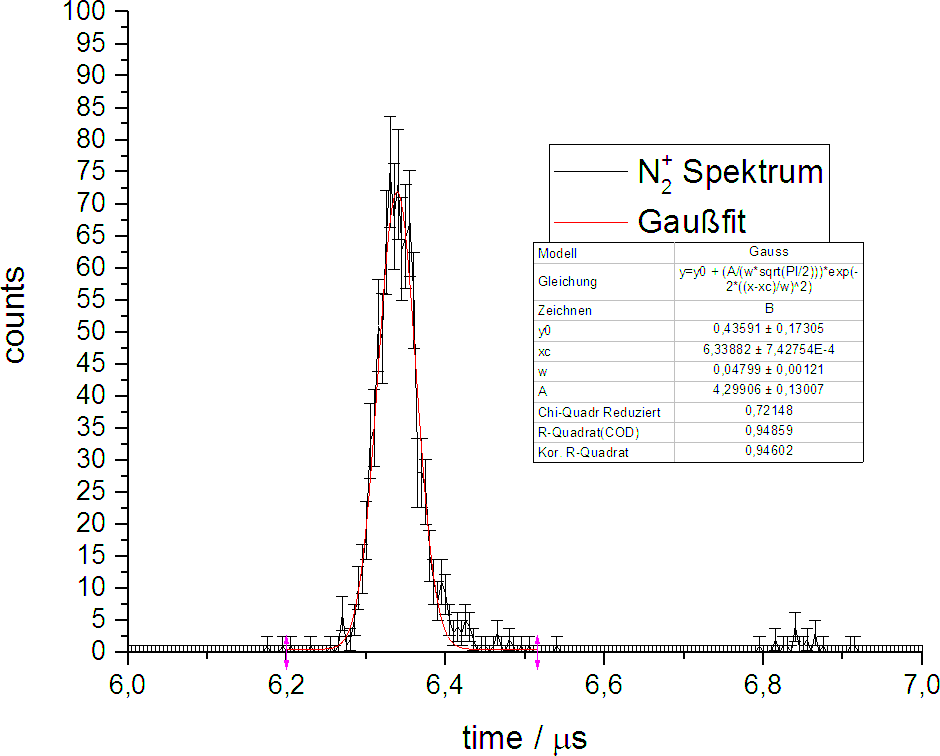
\includegraphics[width=0.8\textwidth]{pics/N2}
		\caption{Flugzeitspektrum für N${}_2^+$-Ionen mit 100 Umläufen im Multireflektron. Der Fehler ist der statistische Fehler der Messwerte. Die durchgelegte Kurve ist ein fehlergewichteter Gaußfit.}
		\label{abb:N2}
	\end{figure}
	
	\begin{figure}[!h]
		\centering
		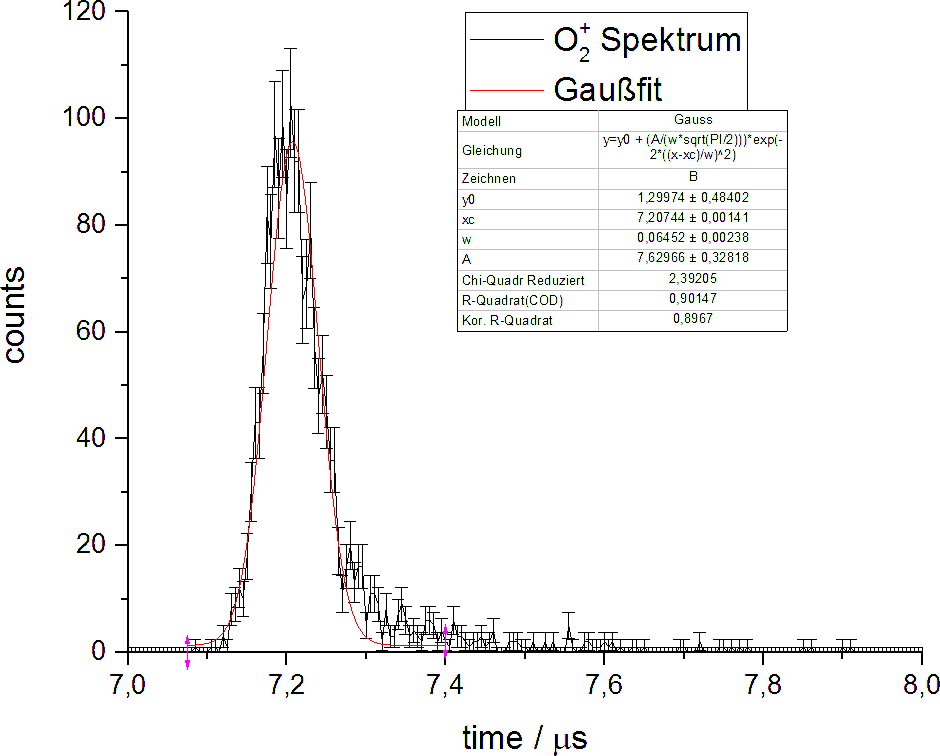
\includegraphics[width=0.8\textwidth]{pics/O2}
		\caption{Flugzeitspektrum für O${}_2^+$-Ionen mit 100 Umläufen im Multireflektron. Der Fehler ist der statistische Fehler der Messwerte. Die durchgelegte Kurve ist ein fehlergewichteter Gaußfit.}
		\label{abb:O2}
	\end{figure}
	
	\begin{figure}[!h]
		\centering
		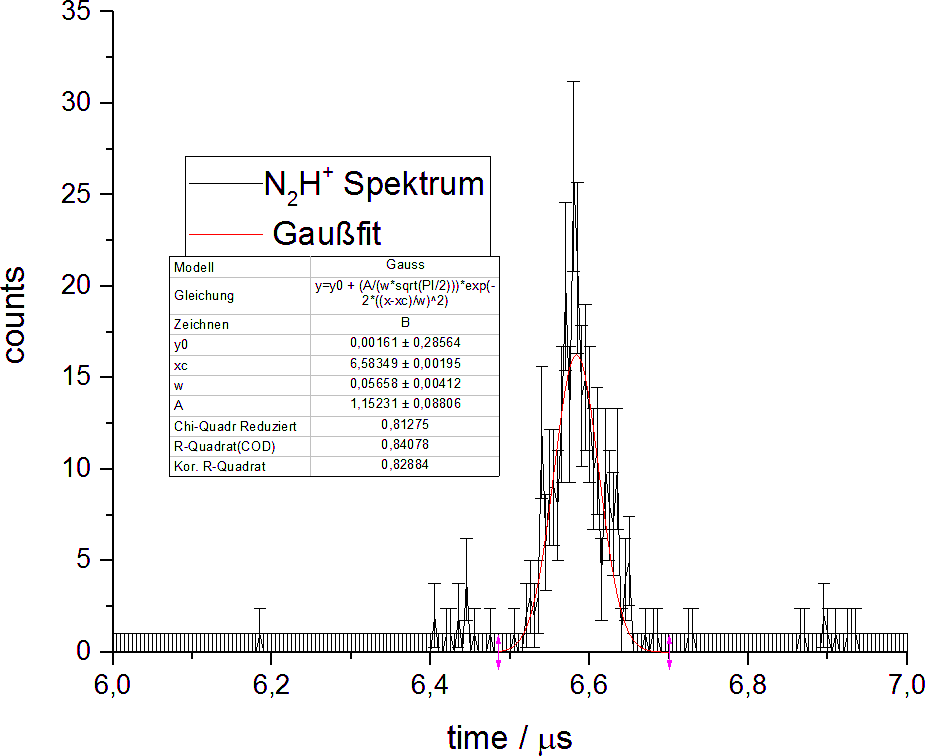
\includegraphics[width=0.8\textwidth]{pics/N2H}
		\caption{Flugzeitspektrum für N${}_2$H$^+$-Ionen mit 100 Umläufen im Multireflektron. Der Fehler ist der statistische Fehler der Messwerte. Die durchgelegte Kurve ist ein fehlergewichteter Gaußfit.}
		\label{abb:N2H}
	\end{figure}
	\clearpage
	
	\subsection{Massenbestimmung von N$_2^+$-Ionen}
	
	Für die berechneten Umlaufzeiten der drei angegebenen Ionen werden nun jeweils drei Spektren bei $100$ Umläufen im Multireflektron aufgenommen. Die Abb.\ref{abb:N2}-\ref{abb:N2H} sind beispielhaft die Spektren der ersten Messung versehen mit einem Gaußfit zur Bestimmung der Position des zeitlichen Peaks $\mu$, sowie dem Faktor $\sigma$, welcher über die Relation
	\begin{equation}
	b_\mathrm{FWHM} = 2 \sigma\sqrt{2 \ln 2}
	\end{equation}
	die Halbwertsbreite $b_\mathrm{FWHM}$ des Peaks angibt. Diese gibt den Fehler für die Positionsbestimmung des Peaks $\Delta t$ an. Die gemessene Positionen der Peaks im Flugzeitspektrum sind in Tab.\ref{tab:zeit} angegeben. Die Massen für O${}_2^+$- und N${}_2$H$^+$-Ionen werden als bekannt angenommen und es werden Werte aus der Literatur verwendet. Weiterhin wird angenommen, dass für die Fehlerrechnung der Fehler dieser Massen also $\Delta m_\mathrm{i} = 0$ gilt.
	\begin{table}[t]
		\centering
		\caption{Die gemessene Peakpostion $\mu$ für verschiedenen Ionensorten.}
		\begin{tabular}{c|c c c} 
			& N$_2^+$ & O$_2^+$ & N$_2$H$^+$ \\
			Nummer & $\mu\,/\,\mathrm{\mu s}$ & $\mu\,/\,\mathrm{\mu s}$ & $\mu\,/\,\mathrm{\mu s}$ \\ \hline
			1 & $6,339$ & $7,807$ & $6,583$ \\
			2 & $6,738$ & $7,208$ & $6,584$ \\
			3 & $6,340$ & $7,208$ & $6,583$ 
		\end{tabular}
		\label{tab:zeit}
	\end{table}
	Aus diesen Werten lässt sich mit \eqref{eq:abszeit} und \eqref{eq:abszeit} die Masse von N$_2^+$ berechnen, wobei $t_1$, $t_2$, $m_1$, $m_2$ die Massen und Flugzeiten der bekannten Ionensorten sind. Weiterhin ist die Zeit $t$ ist die Summe aus der Zeit im Flugzeitspektrum $\mu$, der Zeit in Multireflektron $n\cdot t_\mathrm{U}$ und der Flugzeit von der Ionenquelle bis zum Reflektron, hier als $7\,\mathrm{\mu s}$ gemessen. Der Fehler für die gemessenen Massen ist nach der gaußschen Fehlerfortpflanzung berechnet (Formeln: siehe Anhang). Beides ist in Tab.\ref{tab:masse} angegeben. In der Abb.\ref{abb:masse} sind die Messwerte mit dem jeweiligen absoluten Massenfehler abgebildet. Die erste und die dritte errechnete Masse liegt jeweils weit unterhalb dem erwarteten Massenbereich von $28,05\,\mathrm{u}$. Bei der Messung Tab.\ref{tab:zeit} ist aufgefallen, dass die Peaks der Flugzeitspektren von gleichen Ionensorten bei verschiedenen Messungen weit auseinander liegen. Es ist also anzunehmen, dass bei der Aufnahme der Messdaten ein Fehler unterlaufen ist. Wahrscheinlich wurden die Schaltzeiten für das Reflektron, welche ebenfalls den Start der Datenaufnahme kennzeichnet, zwischen den Messungen falsch gesetzt, was zur Verschiebung der Peaks führte. Die Auswertung wird dennoch fortgesetzt, da die zweite Messung Ergebnisse in einem akzeptablen Massenbereich liefert.
	\begin{figure}[!h]
		\centering
		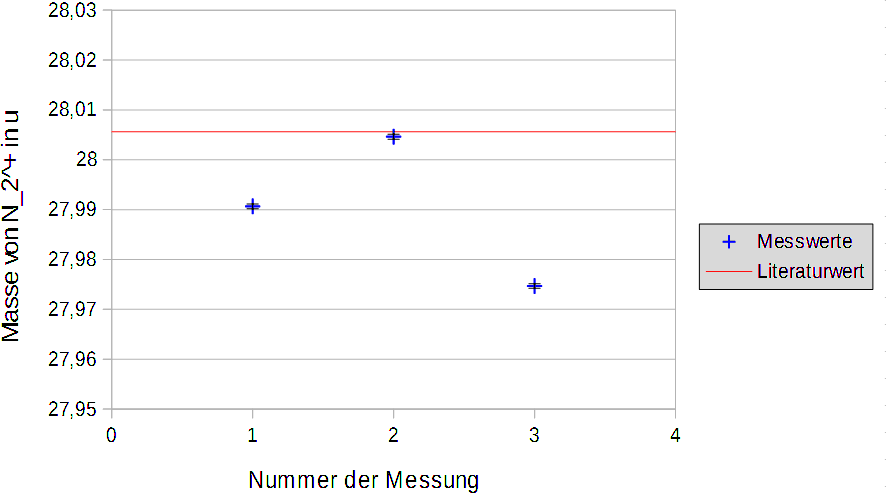
\includegraphics[width = 1.0\textwidth]{pics/Masse}
		\caption{Experimentell errechnete Werte zur Bestimmung der Masse von N$_2^+$-Ionen. Jeder Messpunkt korrespondiert zu einer eigenden Kalibrierung. Die rote Makierung im Graphen repräsentiert den Literaturwert der Ionenmasse. Der Fehler ist durch gaußsche Fehlerfortpflanzung errechnet.}
		\label{abb:masse}
	\end{figure}
	
	
	\begin{table}[h]
		\centering
		\caption{Berechnete Massen $m$ für N$^+_2$-Ionen mit absoluten und relativen Fehler}
		\begin{tabular}{c|c c c} 
			
			Nummer & $m\,/\,\mathrm{u}$ & $\Delta m\,/\,\mathrm{u}$ & $\frac{\Delta m}{m}$ \\ \hline
			1 & $27,991$ & $4,89\cdot 10^{-4}$ & $1,75\cdot 10^{-5}$ \\
			2 & $28,004$ & $5,09\cdot 10^{-4}$ & $1,82\cdot 10^{-5}$ \\
			3 & $27,975$ & $4,43\cdot 10^{-4}$ & $1,58\cdot 10^{-5}$ 
		\end{tabular}
		\label{tab:masse}
	\end{table}
	\clearpage
	
	\subsection{Bindungsenergie und Neutronenseparationsenergie}
	
	Mit der gemessenen Masse von $^{14}$N$^+_2$-Ionen und den Literaturwerten der Protonen-, Neutronenmasse lässt sich die, durch den Massendefekt verursachte, Diskrepanz zwischen der Ionenmasse und der Masse aller Kernteilchen des Ions bestimmen. Die Bindungsenergie $\mathrm{BE}$ ist dann gegeben über die Ruheenergie
	\begin{equation}
	\Delta E = \Delta m\cdot c^2
	\end{equation}
	Die berechneten Bindungsenergien sind in Tab.\ref{tab:bind} mit Vergleich zum Literaturwert aufgeführt. Da die gemessenen Massen i.A. niedriger waren als der Literaturwert ist hier ebenfalls eine Abweichung zu beobachten, jedoch zu höheren Bindungsenergien.
	\begin{table}[h]
		\centering
		\caption{Berechnete Bindungsenergien $\mathrm{BE}$ für $^{14}$N-Atome mit Vergleich zum Literaturwert.}
		\begin{tabular}{c|c} 
			
			Nummer & $\mathrm{BE}\,/\,\mathrm{MeV}$ \\ \hline
			1 & $111,38$ \\
			2 & $104,87$ \\
			3 & $118,81$ \\
			Literatur & $104,66$
		\end{tabular}
		\label{tab:bind}
	\end{table}
	Weiterhin lässt sich auch die Neutronenseparationsenergie $S_\mathrm{n}$ bzw. die Zwei-Neutronenseparationsenergie $S_\mathrm{2n}$ bestimmen. Es gilt
	\begin{align}
	S_\mathrm{n}(N,Z) = \mathrm{BE}(N,Z) - \mathrm{BE}(N-1,Z), \nonumber \\
	S_\mathrm{2n}(N,Z) = \mathrm{BE}(N,Z) - \mathrm{BE}(N-2,Z).
	\end{align}
	Es werden die Separationsenergien für $^{14}$N und $^{15}$N und die Zwei-Neutronenseparationsenergien für $^{16}$N und $^{14}$N bestimmt. Für die unbekannten Bindungsenergien werden Literaturwerte verwendet. Die errechneten Ergebnisse sind in Tab.\ref{tab:sep} aufgeführt. Weiterhin sind die Werte zur ersten und zweiten Messung abseits der erwarteten Literaturwerte.
	\begin{table}[h]
		\centering
		\caption{Berechnete Separationsenergien $S_\mathrm{n}$/$S_\mathrm{2n}$ für N-Atome mit Vergleich zum Literaturwert.}
		\begin{tabular}{c c|c} 
			Isotop & Nummer & $S_\mathrm{n}\,/\,\mathrm{MeV}$ \\ \hline
			& 1 & $4,11$ \\
			$^{15}$N & 2 & $10,62$ \\
			& 3 & $-3,32$ \\ \hline
			$^{15}$N & Literatur & $10,83$ \\ \hline
			& 1 & $17,27$ \\
			$^{14}$N & 2 & $10,76$ \\
			& 3 & $24,71$ \\ \hline
			$^{14}$N & Literatur & $10,56$ \\ \hline
		\end{tabular}
		\quad
		\begin{tabular}{c c|c} 
			Isotop & Nummer & $S_\mathrm{2n}\,/\,\mathrm{MeV}$ \\ \hline
			& 1 & $6,60$ \\
			$^{16}$N & 2 & $13,11$ \\
			& 3 & $-0,83$ \\ \hline
			$^{16}$N & Literatur & $13,32$ \\ \hline
			& 1 & $37,32$ \\
			$^{14}$N & 2 & $30,81$ \\
			& 3 & $44,75$ \\ \hline
			$^{14}$N & Literatur & $30,60$ \\ \hline
		\end{tabular}
		\label{tab:sep}
	\end{table}
	
	\subsection{Fazit}
	
	Es ist trotz einiger Abweichung der Messungen von den Literaturwerten gelungen die Prinzipien des Versuches gut nachzuvollziehen. Eine der Messreihen war sogar erfolgreich und lieferte einen Wert, welcher vergleichbar mit den Literaturangaben ist.

	\clearpage
	\section{Anhang}

	\subsection{Fehlerrechnung}

	Die Fehlerrechnung für den absoluten Massenfehler $\Delta m$ ergibt sich durch gaußsche Fehlerfortpflanzung der Formel \autoref{eq:abszeit} und den Fehlerwerten von $t_1$,$t_2$ und $t$
	\begin{equation}
	\Delta m = \sqrt{\left(\frac{\partial m}{\partial t_1}\cdot \Delta t_1\right)^2+\left(\frac{\partial m}{\partial t_2}\cdot \Delta t_2\right)^2+\left(\frac{\partial m}{\partial t}\cdot \Delta t \right)^2}
	\end{equation}
	Die Ableitungen nach den Referenzmassen $m_1$ und $m_2$ werden als fehlerlos betrachtet, da deren Fehlerwert im Vergleich zu denen des Experimentes hinreichend klein sind. Die partiellen Ableitungen sind gegen durch
	\begin{align}
	\frac{\partial m}{\partial t_1} =& 2 \left(C_\mathrm{ToF}\cdot \Delta_\mathrm{ref}+\frac{\Sigma_\mathrm{ref}}{2}\right) \cdot \Delta_\mathrm{ref}\frac{t_2-t}{\left(t_1-t_2\right)^2} \nonumber \\
	\frac{\partial m}{\partial t_2} =& 2 \left(C_\mathrm{ToF}\cdot \Delta_\mathrm{ref}+\frac{\Sigma_\mathrm{ref}}{2}\right) \cdot \Delta_\mathrm{ref}\frac{t-t_1}{\left(t_1-t_2\right)^2} \\
	\frac{\partial m}{\partial t} =& 2 \left(C_\mathrm{ToF}\cdot \Delta_\mathrm{ref}+\frac{\Sigma_\mathrm{ref}}{2}\right) \cdot \Delta_\mathrm{ref}\frac{1}{\left(t_1-t_2\right)^2} \nonumber
	\end{align}

		\bibliography{all.bib}
		\bibliographystyle{unsrt}

\end{document}